%% abtex2-modelo-trabalho-academico.tex, v-1.9.2 laurocesar
%% Copyright 2012-2014 by abnTeX2 group at http://abntex2.googlecode.com/
%%
%% This work may be distributed and/or modified under the
%% conditions of the LaTeX Project Public License, either version 1.3
%% of this license or (at your option) any later version.
%% The latest version of this license is in
%%   http://www.latex-project.org/lppl.txt
%% and version 1.3 or later is part of all distributions of LaTeX
%% version 2005/12/01 or later .
%%
%% This work has the LPPL maintenance status `maintained'.
%%
%% The Current Maintainer of this work is the abnTeX2 team, led
%% by Lauro César Araujo. Further information are available on
%% http://abntex2.googlecode.com/
%%
%% This work consists of the files abntex2-modelo-trabalho-academico.tex,
%% abntex2-modelo-include-comandos and abntex2-modelo-references.bib
%%

% ------------------------------------------------------------------------
% ------------------------------------------------------------------------
% abnTeX2: Modelo de Trabalho Academico (tese de doutorado, dissertacao de
% mestrado e trabalhos monograficos em geral) em conformidade com
% ABNT NBR 14724:2011: Informacao e documentacao - Trabalhos academicos -
% Apresentacao
% ------------------------------------------------------------------------
% ------------------------------------------------------------------------

\documentclass[
	% -- opções da classe memoir --
	12pt,				% tamanho da fonte
	openright,			% capítulos começam em pág ímpar (insere página vazia caso preciso)
	oneside,			% para impressão sem verso e anverso. Oposto a twoside
	a4paper,			% tamanho do papel.
	% -- opções da classe abntex2 --
	chapter=TITLE,		% títulos de capítulos convertidos em letras maiúsculas
	%section=TITLE,		% títulos de seções convertidos em letras maiúsculas
	%subsection=TITLE,	% títulos de subseções convertidos em letras maiúsculas
	%subsubsection=TITLE,% títulos de subsubseções convertidos em letras maiúsculas
	% -- opções do pacote babel --
	english,			% idioma adicional para hifenização
%	french,				% idioma adicional para hifenização
%	spanish,			% idioma adicional para hifenização
	brazil				% o último idioma é o principal do documento
	]{abntex2-udesc}

% ---
% Pacotes básicos
% ---
\usepackage{lmodern}			% Usa a fonte Latin Modern
\usepackage[T1]{fontenc}		% Selecao de codigos de fonte.
\usepackage[utf8]{inputenc}		% Codificacao do documento (conversão automática dos acentos)
\usepackage{lastpage}			% Usado pela Ficha catalográfica
\usepackage{indentfirst}		% Indenta o primeiro parágrafo de cada seção.
\usepackage{color}				% Controle das cores
\usepackage{graphicx}			% Inclusão de gráficos
\usepackage{microtype} 			% para melhorias de justificação
\usepackage{mathptmx}
\usepackage[singlelinecheck=false]{caption}
% ---

% ---
% Pacotes de citações
% ---
%\usepackage[brazilian,hyperpageref]{backref}	 % Paginas com as citações na bibl
\usepackage[alf,abnt-emphasize=bf,abnt-etal-cite=2]{abntex2cite}	% Citações padrão ABNT
%,abnt-full-initials=yes
%\citeoption{abnt-and-type=&}

% ---
% Pacotes de cor em tabela
% ---
%\usepackage[table]{xcolor}
%\usepackage{array,ragged2e}

% ---
% Pacotes de algoritmos
% ---
\usepackage{listings}

% ---
% Pacotes de simbolos
% ---
\usepackage{pifont}

% ---
% CONFIGURAÇÕES DE PACOTES
% ---

% ---
% Configurações do pacote backref
% Usado sem a opção hyperpageref de backref
%\renewcommand{\backrefpagesname}{Citado na(s) página(s):~}
% Texto padrão antes do número das páginas
%\renewcommand{\backref}{}
% Define os textos da citação
%\renewcommand*{\backrefalt}[4]{
%	\ifcase #1 %
%		Nenhuma citação no texto.%
%	\or
%		Citado na página #2.%
%	\else
%		Citado #1 vezes nas páginas #2.%
%	\fi}%
% ---% ---
% Configurações do pacote listings
\lstdefinelanguage{portugol}
  {morekeywords={Algoritmo,Var,inteiro,Inicio,escreva,Fim}
}
\lstset{
  breakatwhitespace=false,
  breaklines=true,
  escapeinside={\%*}{*)},
  keywordstyle=\bfseries\color{black},
  language=portugol,
  showstringspaces=false,
}
% ---% ---

% ---
% Informações de dados para CAPA e FOLHA DE ROSTO
% ---
\titulo{Interpretador de Algoritmos Portugol em HTML5}
\autor{Gilberto Tavares}
\cidade{São Bento do Sul}
\uf{SC}
\local{\inserecidade, \insereuf}
\data{2016}
\orientador{Dr. Luiz Cláudio Dalmolin}
\instituicao{Universidade do Estado de Santa Catarina - UDESC}
\centro{Centro de Educação do Planalto Norte - CEPLAN}
\curso{Bacharelado em Sistemas de Informação}
\tipotrabalho{Trabalho de Conclusão de Curso}
% O preambulo deve conter o tipo do trabalho, o objetivo,
% o nome da instituição e a área de concentração
\preambulo{Trabalho de Conclusão apresentado ao Curso de Bacharelado em Sistemas
de Informação, da Universidade do Estado de Santa Catarina, como requisito para
a obtenção do grau de Bacharel em Sistemas de Informação}
% ---

% ---
% Configurações de aparência do PDF final

% alterando o aspecto da cor azul
%\definecolor{blue}{RGB}{41,5,195}
\definecolor{blue}{rgb}{0,0,0}

% informações do PDF
\makeatletter
\hypersetup{
     	%pagebackref=true,
		pdftitle={\@title},
		pdfauthor={\@author},
    	pdfsubject={\imprimirpreambulo},
	    pdfcreator={LaTeX with abnTeX2},
		pdfkeywords={lógica da programação}{algoritmos}{portugol}{interpretador}{html5},
		colorlinks=true,       		% false: boxed links; true: colored links
    	linkcolor=black,          	% color of internal links
    	citecolor=blue,        		% color of links to bibliography
    	filecolor=magenta,      		% color of file links
		urlcolor=blue,
		bookmarksdepth=4
}
\makeatother
% ---

% ---
% Espaçamentos entre linhas e parágrafos
% ---

% O tamanho do parágrafo é dado por:
\setlength{\parindent}{1.3cm}

% Controle do espaçamento entre um parágrafo e outro:
\setlength{\parskip}{0.2cm}  % tente também \onelineskip

% ---
% compila o indice
% ---
\makeindex
% ---

% ----
% Início do documento
% ----
\begin{document}
% Retira espaço extra obsoleto entre as frases.
\frenchspacing

% ----------------------------------------------------------
% ELEMENTOS PRÉ-TEXTUAIS
% ----------------------------------------------------------
% \pretextual

% ---
% Capa
% ---
% TODO PRINT Descomentar
%\imprimircapa
% ---

% ---
% Folha de rosto
% (o * indica que haverá a ficha bibliográfica)
% ---
%\imprimirfolhaderosto*
% TODO PRINT Descomentar
%\imprimirfolhaderosto
% ---

% Folha de Aprovação
% TODO PRINT Descomentar
%
% ---
% Inserir folha de aprovação
% ---

% Isto é um exemplo de Folha de aprovação, elemento obrigatório da NBR
% 14724/2011 (seção 4.2.1.3). Você pode utilizar este modelo até a aprovação
% do trabalho. Após isso, substitua todo o conteúdo deste arquivo por uma
% imagem da página assinada pela banca com o comando abaixo:
%
% \includepdf{folhadeaprovacao_final.pdf}
%
\begin{folhadeaprovacao}

  \begin{center}
    {\ABNTEXchapterfont\bfseries\MakeTextUppercase{\imprimirautor}}

    \vspace*{\fill}\vspace*{\fill}
    \begin{center}
      \ABNTEXchapterfont\bfseries\MakeTextUppercase{\imprimirtitulo}
    \end{center}
    \vspace*{\fill}

   \end{center}

  \noindent
  \imprimirpreambulo

  \vspace*{\fill}

  \noindent
  {\bfseries Banca Examinadora}

  \vspace*{\ABNTEXsignskip}

  \setlist[description]{font=\normalfont}

  \begin{description}[labelindent=0pt,labelwidth=4cm] %label={\textnormal},
    \item[Orientador:]
    \assinaturaorientador{\textbf{\href{http://lattes.cnpq.br/7393306373465290}{\imprimirorientador} \\ Universidade do Vale do Itajaí}}
  \end{description}

  \setlist[description]{font=\bfseries}

  \begin{description}[labelindent=0pt,labelwidth=4cm] %label={\textnormal},
    \item[Membros:]
    \vspace*{\ABNTEXsignskip}
    \assinaturaorientador{\textbf{\href{http://lattes.cnpq.br/3985354928735296}{Dr. Nilson Ribeiro Modro} \\ Universidade Federal de Santa Catarina}}
    \item[]
    \vspace*{\ABNTEXsignskip}
    \assinaturaorientador{\textbf{\href{http://lattes.cnpq.br/3317225251677148}{Ma. Nelcimar Ribeiro Modro} \\ Universidade Federal do Paraná}}
  \end{description}

   \begin{center}
    \vspace*{0.5cm}
    \inserecidade~\insereuf, 29/11/2016
    \vspace*{1cm}
  \end{center}

\end{folhadeaprovacao}
% ---


% Dedicatória, Agradecimentos, Epígrafe - Elementos Pré textuais opcionais
% TODO PRINT Descomentar
%
% Dedicatória

% ---
% Dedicatória
% ---
\begin{dedicatoria}
   \vspace*{\fill}
   \hspace{.45\textwidth}
   \begin{minipage}{.5\textwidth}
      \SingleSpacing
Dedico este aos meus familiares falecidos:
% Talvez reticências ...

Meu irmão que sempre apoiou minha formação
superior e carreira até oferecendo certa
colaboração financeira.

E ainda mais recente meu pai que financiou
meu pré ingresso e não pude compartilhar
com ele esta conquista.
   \end{minipage}
	\vspace*{\fill}
\end{dedicatoria}
% ---


% ---
% Agradecimentos
% ---
\begin{agradecimentos}

A minha mãe me apoiou em minha decisão de cursar faculdade noutra cidade. E sempre que possível (mesmo com dificuldade) ajudou como pode: com móveis para meu primeiro quarto, algumas compras de mercado e algum dinheiro quando ficava mais crítico. Inclusive isso tudo pode ter sido um dos motivos da decisão dela em vender o imóvel em que morávamos.

A toda a família Lischka que me acolheu inicialmente como hóspede na residência do casal Arnaldo e Jacira (prima da minha mãe). Foi também na empresa familiar deles, juntos com seus filhos, que tive meu primeiro emprego na cidade e me foi cedido para moradia um quartinho e dependências junto à empresa.

Ao meu irmão que me empregou as sábados e minhas cunhadas que me hospedavam, além de amigos. A todos os motoristas que me deram carona, economizando assim a passagem para que eu pudesse voltar com uma grana a mais do final de semana.

A todos os meus amigos de moradia que tiveram que me aguentar nas repúblicas que habitei, especialmente à mais recentemente extinta ``Mansão Amarela''.

A Joseli que sua experiência passando pelo mesma situação de fim de curso foi de grande ajuda. Também seu apoio e motivação, bem como dos meu amigos de infância José e Rafael que fizeram o mesmo.

A toda a experiência social, esportiva e de conheciento que as confraternizações com outros academicos, Jiudesc e os vários Latinoware proporcionaram.

As empresas Hardline e Xthor que me ofereceram estágio e emprego respectivamente. Principalmente a segunda, na qual todo aprendizado e parceria com o Richard levou ao meu crescimento profissional, acadêmico e pessoal.

Sem esquecer é claro das minhas garrafas térmicas, que mantiveram tanto café quentinho quanto suco de guaraná gelado para embalar as noites dedicadas a esta realização.


\end{agradecimentos}
% ---

% Epígrafe

% ---
% Epígrafe
% ---
\begin{epigrafe}
    \vspace*{\fill}
   \hspace{.45\textwidth}
   \begin{minipage}{.5\textwidth}
      \SingleSpacing

% No idioma de origem
% ``Most good programmers do programming not
% because they expect to get paid or get adulation
% by the public, but because it is fun to program..''

% Tradução original
% ``A maioria dos bons programadores programam não
% porque esperam ser pagos ou adulados pelo público,
% mas porque é divertido programar.''

{\small``A maioria dos bons programadores programa
não por esperar ser pago ou adulado pelo público,
mas porque é divertido programar.''  (tradução nossa)

\vspace{\onelineskip}

Linus Torvalds}
   \end{minipage}
	\vspace*{\fill}
\end{epigrafe}
% ---



% Resumos (em português e pelo menos em inglês)
% TODO PRINT Descomentar
%
% ---
% RESUMOS
% ---

% resumo em português
%MODRO: Resumo Monografia
%Qual o problema? Qual a dificuldade atual?
%Porque da solução?
%Como desenvolvido?
%Diagramas modelagem?
%Tempo de desenvolvimento?
%Processo de aprendizado?
%Ferramentas utilizadas?
%Market share?
%Funcionalidades?
%Onde testado?
%Onde utilizado?
%Casos de uso? Opiniões?
%Documentação / Projeto?
\begin{resumo}
Trata-se do estudo das opções para prática computacional no processo de ensino e aprendizagem, sugerindo um conceito de ferramenta que diferente das existentes, pois permite acesso via navegador de internet sem instalação ou download adicional. Vários conceitos são apresentados sobre algoritmos como: sua estrutura e seus tradutores, sejam eles compiladores ou interpretadores. Mas para o foco do trabalho apenas algoritmo com simples impressão em tela foi implementado, permitindo demonstrar seu diferencial que além de acesso nativo via navegador o pode ser utilizado sem conexão com a internet. Sendo o problema a atual dificuldade de iniciar a execução do programa para a prática durante o aprendizado de algoritmos, vem se propor esta solução para acesso simplifica independente da plataforma ou dispositivo do aluno. Foi desenvolvido utilizando da ferramenta utilizada nesta instituição por alguns professores como modelo, ela foi repensada modo minimalista quanto sua interface, desse pensamento o diagrama de caso de uso foi obtido. Foi necessário um processo de aprendizado sobre compiladores por não termos neste curso ainda alguma disciplina que aborde este tema. Se de modo ininterrupto pode-se concluir como tempo total de desenvolvimento três meses. Foram utilizadas técnicas de vanguarda para funcionamento em navegadores modernos, dentre essas os últimos padrões da linguagem de programação ECMAScript (popularmente JavaScript). Nessa linguagem foram encontrados componentes de código livre: Acorn e JS-Intrepreter para a análise léxico-sintática e execução semântica respectivamente, além do Ace como editor de texto.

\vspace{\onelineskip}
\textbf{Palavras-chaves}: Lógica da programação. Algoritmos. Portugol. Interpretador. HTML5.
% ensino, aprendizagem
\end{resumo}

% resumo em inglês
%\begin{resumo}[Abstract]
%\begin{otherlanguage*}{english}
%
%\vspace{\onelineskip}
%\textbf{Key-words}: Programming logic. Algorithms. Portugol. Interpreter. HTML5.
%% teaching, learning
%\end{otherlanguage*}
%\end{resumo}


% Lista de Ilustrações
% TODO PRINT Descomentar
%

% ---
% inserir lista de ilustrações
% ---
\pdfbookmark[0]{\listfigurename}{lof}
\listoffigures*
\cleardoublepage
% ---


% Lista de Siglas
% TODO PRINT Descomentar
%
% ---
% inserir lista de tabelas
% ---
\pdfbookmark[0]{\listtablename}{lot}
\listoftables*
\cleardoublepage
% ---


% Lista de Siglas
% TODO PRINT Descomentar
%
% ---
% inserir lista de abreviaturas e siglas
% ---
\begin{siglas}
%  \item[CSS] Hyper Text Markup Language
  \item[HTML] \textit{HyperText Markup Language}
  \item[SW] \textit{Service Workers}
  \item[UAL] UNESA \textit{Algorithmic Language}
  \item[UNESA] Universidade Estácio de Sá
\end{siglas}
% ---


% ---
% inserir o sumario
% ---
\pdfbookmark[0]{\contentsname}{toc}
\tableofcontents*
\cleardoublepage
% ---



% ----------------------------------------------------------
% ELEMENTOS TEXTUAIS
% ----------------------------------------------------------
\textual


% Capítulo 1 - Introdução

% ----------------------------------------------------------
% Introdução (exemplo de capítulo sem numeração, mas presente no Sumário)
% ----------------------------------------------------------
\chapter{Introdução}
%\addcontentsline{toc}{chapter}{Introdução}
% ----------------------------------------------------------

\ifdraft{\color{green}}{}A base da programação é ensinar a máquina realizar determinada tarefa, para que isso seja possível é necessário que o usuário comunique-se com a máquina, numa linguagem que ela entenda, a linguagem de programação. A construção da linguagem de programação envolve ações definidas em passos que se deseja que a máquina execute, a estes passos damos o nome de algoritmos. Para isso pode-se dizer que independente do paradigma utilizado no processo de desenvolvimento ele envolve algoritmos \cite{medeiros2015}.

Algoritmos podem não necessariamente serem computacionais, já que são um conjunto de passos finitos. Analogias simplistas são os ingredientes e modo de preparo de uma receita ou instruções para uma tarefa do cotidiano, como a troca de um pneu furado em um automóvel \cite{medina2006etal}. Porém se tratando de computação deve ter maior formalidade, seguindo uma linguagem pois diferente do ser humano uma máquina não é tão interpretativa. Desconsideradas aqui inteligências artificiais que são desenvolvidas por algoritmos para terem  comportamento de compreensão humana. Isto pode ser analogamente algo como não entender idioma estrangeiro e as instruções estarem nesta linguagem. Porém em informática isso tem que ser mais especificado com palavras ou caracteres predeterminados de início e fim, de blocos, repetições, etc \cite{dershem1990etal}.

Sendo o berço mais popular da informática os Estados Unidos da América e seus criadores em muitos casos dessa origem ou de países com mesmo idioma as primeiras linguagens de computação e a maioria delas são em inglês \cite{sebesta2009}. Isso muda quando falamos do Portugol que possui variações, mas resumidamente sua origem vem como uma tradução de uma linguagem de programação simples e comum, com seus termos no idioma nativo do Brasil.

Tendo como foco o aprendizado de algoritmos para uma boa fundamentação de futuros programadores ou profissionais da área, muitas vezes a facilidade com o inglês não é algo comum em nosso país, a linguagem Portugol se torna um artifício vantajoso \cite{jesus2004etal}.  Neste sentido já é utilizado pela maioria dos professores do Centro de Educação Superior do Planalto Norte (CEPLAN) da Universidade do Estado de Santa Catarina (UDESC) livro texto e software para a prática do aprendizado de algoritmos em Portugol.

Porém quando o software é exclusivo para uso em um único sistema operacional, instalações que podem não serem simples ou mesmo não acessível de outros dispositivos, passa a complicação adicional ao aluno iniciante. Por isso o protótipo propoẽ ser acessível em qualquer navegador web, desde que alinhado com as tecnologias mais recentes. Sem contudo deixar de permitir que possa permanecer a prática de algoritmos quando não houver conexão com a internet.


{\color{green}\section{Objetivos do Trabalho}}

\ifdraft{\color{green}}{}\subsection{Objetivo Geral}

Apresentar o conceito de ferramenta computadorizada para se tornar referência
em criação, edição, visualização e interpretação de algoritmos em
pseudolinguagem, como alternativa às existentes. Sendo seu diferencial o acesso
a partir de navegadores Web por ser em HTML5. Inclusive acessível quando uma
conexão com a internet esteja indisponível.
% NOTE \footnote{Desde que haja ao menos um acesso anterior.}

\subsection{Objetivos Específicos}

Visando atingir o objetivo geral em sua totalidade lista-se a seguir objetivos
específicos de modo sucinto:

\begin{itemize}
  %\setlength\itemsep{0em}
  \item Desenvolver o protótipo, sendo seu código fonte aberto e
  disponível para que outros possam manter, ampliar e evoluir a aplicação;
  \item Fazê-lo compatível com sintaxe UAL e mínimo produto viável para as
  primeiras lições de ensino aprendizagem;
  \item Permitir o acesso via navegadores web modernos, sem necessidade de
  instalações complementares;
  % Para isso utilizar HTML5 que pode ser descrito como o uso de somente linguagem de programação ECMAScript (popularmente Javascript), e para inferface gráfica essencialmente a combinação de HTML (abreviação para a expressão inglesa HyperText Markup Language, que significa Linguagem de Marcação de Hipertexto) e de estilização em Cascading Style Sheets (CSS) em suas versões recomendáveis pelo World Wide Web Consortium (W3C).
  \item Aplicar aprimoramentos introduzidos na versão 5 do HTML
  (\textit{HyperText Markup Language}) para uso sem conexão com a internet.
\end{itemize}\color{black}


\section{Justificativa do Trabalho}

\ifdraft{\color{green}}{}Praticar em \textit{software} à abstração em papel auxilia e muito no processo de ensino e aprendizagem, em algoritmos além do pensamento lógico por etapas já pode ser desenvolvido e descrito para o repasse a um computador.
``O Aprendizado de algoritmos não é uma tarefa muito fácil, só se consegue através de muitos exercícios'' \cite[p.~1]{lopes2002etal}.

Para esse ensino é essencial conhecer dois conceitos principais lógica de programação e algoritmos. Primeiramente é apresentado um paralelo de situações do cotidiano com algoritmos, ao efetuar comparações de instruções passo a passo realizadas diariamente, como fritar um ovo ou trocar um pneu de automóvel. A seguir inicia-se a aplicação de linguagem estruturada em português para descrição dos algoritmos. Em alguns casos, utiliza-se de linguagens em inglês, mo por exemplo, Pascal. Há professores que preferem usar pseudo linguagem em português somente ``em papel'', iniciando a codificação diretamente em linguagem C. Tem-se inclusive, também ``em papel'', de analisar e interpretar os passos do algoritmo para saber quais serão os valores em memória e a saída na tela.

Simultaneamente, com a prática escrita, sem software específico, pode-se simular os mesmos algoritmos em interpretador ou compilador. Sendo em um interpretador sua construção dividida em partes, cada uma com uma função específica. Geralmente identifica-se: o analisador léxico, o analisador sintático, o analisador semântico, e o resultado de saída. Caso seja um compilador há, ao invés de resultado de saída, o gerador de código, que transforma o programa em linguagem de máquina composta de 0s e 1s \cite{delamaro2004}.

Diante do exposto, este trabalho justifica-se pelo empenho em facilitar o processo de aprendizagem de algoritmos, desenvolvendo um um programa em navegador via Internet, fazendo com que seja desnecessária a instalação do programa,  podendo ser acessado a partir de qualquer computador, com o objetivo que os exercícios sejam resolvidos com maior praticidade\color{black}


\section{Estrutura do Trabalho}


No presente trabalho apresentar-se-á a forma de desenvolvimento do primeiro
módulo, o interpretador, a interface com o usuário e diretrizes para a
execução do módulo restante que não será executado, e que poderão ser ampliados
a partir desta base de estudo e conhecimentos aplicados no presente projeto.

O restante do projeto está organizado da seguinte forma: no capítulo 2 é
relatada a forma como foi idealizado o desenvolvimento da ferramenta proposta;
no capítulo 3 descreve-se como o módulo interpretador está sendo desenvolvido;
nos capítulos 4 e 5 são apresentadas as diretrizes que serão seguidas para os
desenvolvimentos dos módulos Interface Homem-Máquina e sugestão de Sistema de
Informação para o Professor, respectivamente; no capítulo 5 são apresentados as
considerações finais.



% Capítulo 2 - Fundamentação Teórica
\ifdraft{\color{green}}{}\chapter{Fundamentação Teórica}

Para o entendimento e desenvolvimento da proposta conforme explícita nos objetivos gerais e específicos, alguns conceitos teóricos devem ser dispostos. Algoritmos do conceito ao modelo utilizado, variações de modelos algorítmicos e outros ambientes de estudo, ensino ou prática.

\section{Linguagem Natural}

Com menor rigidez do que se faz necessário para uma máquina, esses conjuntos também podem ser descritos em uma linguagem humanamente mais natural. Numa conversa ou em uma explicação de rota de um destino ou uma receita culinária o entendimento ocorrerá. Por depender de formalidade e buscando a aproximação com a rigidez das linguagens de programação utiliza-se o idioma estruturado. Em nosso caso o português estruturado, mas há também o inglês estruturado e certamente outras \ifdraft{\cite{citar}}{\cite{medina2006etal}}.

\section{Programas de Computador}

%\textrightarrow
Sua estrutura é E$\,\to\,$P$\,\to\,$S (entrada-programa-saída), podendo não haver argumentos de entrada. Exemplo, um programa após compilado pode receber em sua execução como argumento um número inteiro para resultar em sua raiz quadrada, ou outro sem receber argumento já tenha a raiz quadrada de um número pré definido \ifdraft{\cite{citar}}{\cite{medina2006etal}}.

\section{Pseudo código ou linguagem}

Visando ser uma ponte entre a linguagem natural e as linguagens de programação temos as pseudo-linguagem. Notadamente Portugol é evidenciada como a solução, pois desde \citeonline{saliba1992} é confirmada sua ampla utilização. Porém não há uma padronização existindo inúmeras variações, no entanto com muitas semelhanças entre si \ifdraft{\cite{citar}}{\cite{medina2006etal}}.

\section{Algoritmos}

A última das notas de Ada Lovelace, que foram republicadas em 1953\nocite{1253887}, apresenta os
primeiros conceitos sobre programação, descrevendo um algoritmo. Desde então
estes foram difundidos, sendo utilizados até a atualidade
\cite{santiago2003etal}.

Conforme \citeonline{medina2006etal} algoritmo é um termo mais amplo, sendo inclusive destinado a outras áreas e finalidades além da programação. As encontradas na literatura são interpretativas porém todas chegam ao mesmo resultado, um {\bfseries conjunto de instruções para a resolução de uma situação}.

Como algoritmo é um conjunto de instruções pode-se dizer então que ele é também um programa de computador, apresentando um conjunto de operações e instruções específicas para a saída que se pretende \cite{medina2006etal}.

%Alguns autores afirmam que estas instruções mas afirmações são determinam instruções são passos detalhadas para a solução ou mesmo que tipo de situação, se especificamente um problema ou tarefas em geral.

%Como podemos perceber, um programa nada mais é que um tipo de algoritmo. Sua particularidade é que suas operações são específicas para o computador e restritas ao conjunto de instruções que o processador pode executar. Podemos considerar esse conjunto de instruções como a primeira linguagem de programação do computador, também chamada de linguagem de máquina.

Para \citeonline{santiago2003etal} a estruturação do algoritmo com suas representações é dada da seguinte forma:

\begin{itemize}

\item Tipos de Dados: tipo de valores inserido nas variáveis;
\item Variáveis: armazenagem na memória principal;
\item Atribuições: definir valor numa variável;
\item Operações aritméticas: utilizadas em cálculos entre números e variáveis;
\item Estruturas de Controle: para fluxo, com desvio condicional e laços de repetição;
\item Operações relacionais: estabelecem relação entre comparações;
\item Vetores: variáveis com único nome, contendo um índice de posições.

\end{itemize}

% Com base nos dois parágrafos abaixo, reescrever utilizado como referência de embasamento os autores \cite{santiagodazzi2003}

%Um algoritmo consiste em um procedimento, composto por uma série de passos
%utilizados para resolver problemas computacionais específicos, que a partir do
%processamento comdados de entradas irá gerar dados de saídas (CORMEN et al,
%1999).

%Para efetuar funcionalidade em um algoritmo e verificar a integridade deste é
%necessário testar o algoritmo verificando o conteúdo das variáveis passo a
%passo. Para efetuar esta tarefa costuma-se utilizar o Teste de Mesa. Também
%chamado Teste Exaustivo, executa para cada instrução, uma verificação, e a
%amostragem do conteúdo das variáveis utilizadas no algoritmo, permitindo que o
%programador visualize o comportamento de todo o processo. Isso permite não
%apenas a comprovação do correto funcionamento, mas também detectar e corrigir
%com facilidade eventuais erros.

\section{Tradutores}
%Compiladores e Interpretadores

%Um compilador traduz um programa descrito em uma linguagem de alto nível, mais
%adequada aos seres humanos, para os códigos em uma linguagem de máquina, que
%podem ser executados por um processador. Grosso modo, o processo de
%compilação pode ser descrito como contendo as seguintes etapas: análise léxica, análise
%sintática, análise semântica e geração de código.\cite{barbosa2009etal}

Neste caso tradutor é um programa com capacidade de fazer leitura em uma linguagem e traduzir para outra equivalente. Conforme \citeonline{aho2007etal} existem dois principais tipos de tradutores: compiladores e interpretadores. Ilustrada a diferenciação entre elas na figura \ref{fig:versus}, a partir de uma mesma fonte o compilador à esquerda e o interpretador a direita demonstra que o interpretador tem sua execução traduzindo diretamente cada instruçao.

\begin{figure}[h]
  \caption{\ifdraft{\color{green}}{}Compilador \textit{versus} Interpretador}\label{fig:cversus}
  \centering
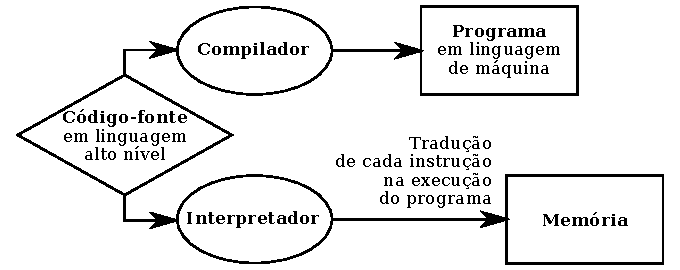
\includegraphics[width=\textwidth,height=10cm,keepaspectratio]{figures/compilador-interpretador.pdf}
  \caption*{\ifdraft{\color{green}}{}\footnotesize Fonte: Produção do autor, adaptado de \citeonline{medina2006etal}.}
\end{figure}

Passando por um processo de entendimento de elementos mínimos no código, ignorando outros e agrupando em símbolos especificados, a compilação se inicia. Além dessa análise também é necessária a verificação se esses grupos estão em ordem ou outros erros possíveis. \citeonline{delamaro2004} descreve que código fonte de entrada termina tendo como saída o programa objeto, o compilador converte a linguagem simples em uma linguagem entendida pela máquina. Explicado o processo do compilador de maneira simples e objetiva é preciso ainda nomear tecnicamente além de expor sua etapas, sendo suas principais as análises: Léxica, Sintática e Semântica.

\begin{figure}[h]
  \caption{\ifdraft{\color{green}}{}Etapas de um compilador}\label{fig:compilador}
  \centering
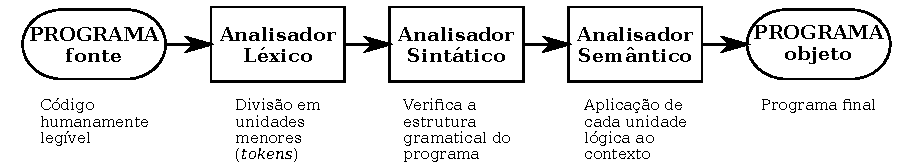
\includegraphics[width=\textwidth,height=10cm,keepaspectratio]{figures/etapas-compilador.pdf}
  \caption*{\ifdraft{\color{green}}{}\footnotesize Fonte: Produção do autor, adaptado de \citeonline{ferrandin2005etal}.}
\end{figure}

%\subsection{Análise Morfológica}
%
\subsection{Análise Léxica}

Também denominada \textit{scanner} cita \citeonline{aho2007etal} como sendo onde elementos mínimos, \textit{tokens}, são identificados. Cada letra, número e outros caracteres (como pontuação e demais símbolos)  além do espaço após reconhecidos são então agrupados com lexemas em: palavras reservadas, comandos, conjunto de texto, nome de variáveis, inícios e fins do algoritmos ou de blocos nele. No quadro \ref{qua:print} é dado uma linha de algoritmo para na tabela \ref{tab:lexemas} apresentar os lexemas indentificados.

\begin{quadro}[h]
\centering
  \caption{Exemplo para entendimento de tradutor}\label{qua:print}
\begin{lstlisting}[language=ual,frame=single]
  imprima "Aprendendo Algoritmo";
\end{lstlisting}
  \caption*{\ifdraft{\color{green}}{}\footnotesize Fonte: Produção do autor.}
\end{quadro}

\begin{table}[h]
\centering
  \caption{Lexemas encontrados no exemplo preposto}\label{tab:lexemas}
\begin{tabular}{ c | l }\hline
\textbf{Lexema} & \textbf{Classificação} \\ \hline
\texttt{imprima} & comando de impressão \\ \hline
\texttt{"Aprendendo Algoritmo"} & conjunto literal de texto \\ \hline
\texttt{;} & caractere de encerramento de expressão \\ \hline
\end{tabular}
  \caption*{\ifdraft{\color{green}}{}\footnotesize Fonte: Produção do autor.}
\end{table}

\subsection{Análise Sintática}

Ou \textit{scanner}, recebe a sequência de lexemas da análise anterior e determina se são elementos estruturais pertencentes à linguagem desejada, exposto por \citeonline{delamaro2004}. São essas estruturas: expressões aritméticas, comandos de atribuição ou declarações de procedimentos e as relações entre eles, garantindo que seja correto sintaticamente. Considerendo o mesmo exemplo do quadro X, a árvore que seria produzida é ilustrada na Figura X abaixo.

\subsection{Análise Semântica}

Esta análise verifica o ``significado'' de comandos, ao tratar de aspectos relacionados a sua ordem para que tenha sentido dentro do definidido pela gramática da linguagem para a correta execução. É possível que um programa esteje em acordo com a sintáxe gramatical, porém apresente erros quanto a semântica. Por exemplo se só for possível imprimir conjuntos literais de texto, variáveis, conjuntos dessas ou operações aritméticas entre parênteses e for criado como impressão direta de um número.

\section{Ferramentas Existentes}
% Ferramentas para prática de algoritmos

\begin{itemize}

\item \textbf{ILA + AMBAP}: Desenvolvida por \citeonline{evaristo2000} o Interpretador de Linguagem Algorítmica (ILA) é um intepretador via linha de comando no qual o AMBAP - AMBiente para Aprenzidadeo e Programaçao utitilizou em seu editor \cite{citar}.

\item \textbf{UAL + EditorUAL}: Desenvolvido em um trabalho na UNESA era basicamente compilador via linha de comando, desenvolvido em Haskel para linux. Ele foi posteriormente portado para Windows, e neste recebeu um editor próprio Editor UAL \cite{citar}.

Todos os algoritmos propostos para execução computadorizada são impressos nesta sintaxe variante do Portugol. Porém para a desenvolvida por \citeonline{evaristo2000} o Interpretador de Linguagem Algorítmica (ILA) \cite{citar}.

\item \textbf{VisuAlg}: Desenvolvida por Claudio Morgado de Souza profissional programador e analista bem como professor universitário, é utilizada tanto em cursos técnicos quanto em meio universitário. A facilidade de obtenção do seu executável para Windows (não necessária instalação), documentação e simplicidade, sem perder funções úteis para iniciantes, são grandes atrativos \cite{souza2013etal}.

\item \textbf{Web Portugol}: Desenvolvida por pesquisadores na UNIVALI permite o acesso via navegadores que tenham integração com Java, desde que o mesmo também esteja instalado no computadors \cite{souza2013etal}.

\item \textbf{Construtor}: Desenvolvido pelo Centro Educacional de Informática Aplicada do SENAC (Rio de Janeiro), é a primeira ferramenta encontrada para uso em plataforma Windows e tem a vantagem acompanhar o livro ``Construção de Algoritmos`` de \citeonline{fernandes1999etal}.

\end{itemize}

Abaixo um comparativo de pontos que ressaltam como fatores determinantes em escolha da opção ao uso.

\begin{quadro}[h]
\centering
  \caption{Comparativo das ferramentas}\label{qua:compare-tools}
\begin{tabular}{| r | l | l | l | l |}\hline
& VisuAlg & Web Portugol & Portugol/Plus & Contrutor \\ \hline
Plataforma & Windows & Web (Java Applet) & DOS & Windows \\ \hline
Licença & \textit{freeware} & \textit{open source} & \textit{open source} & \textit{open source} \\ \hline
Instituição &  & UNIVALLI & UNOESC & SENAC \\ \hline
Linguagem &  & Java &  &  \\ \hline
\end{tabular}
  \caption*{\ifdraft{\color{green}}{}\footnotesize Fonte: Produção do autor.}
\end{quadro}

Desenvolvida por \citeonline{esmin1998} quando vinculado a UNOESC o \textbf{Portugol/Plus} é a mais antiga opção encontrada no Brasil. Merecendo destaque por ser comumente referenciada por outros autores, inclusive quando tratam sobre desenvolvimento de novas soluções. Porém por ser em plataforma \textit{Disk Operating System (DOS)}, inclusive com interface gráfica foi desconsiderada no levantamento acima.

Ao delimitar a quantidade de itens outras também não foram listadas, alguns casos o acesso ao programa para testes não estava disponível ou menor relevância na literatura. No entanto  merecem menção: \textbf{PascalX}, por Athur Vargas Lopes da ULBRA; \textbf{Web-UNERJOL}\nocite{ferrandin2015}, utilizando UNERJOL os dois por acadêmico na UNERJ com colaboração.
%PascalX\nocite{http://www.ulbra.tche.br/~avl/home.htm}

Outras mais não foram consideradas por fugirem do escopo ao utilizar robótica, jogos, foco em estrutura de dados ou similares: Guido VanRobot, Robot Prog, Kids Ruby, Fut Code, TBC-AED. Eram pretendidas somente ferramentas com pseudo-linguagem algorítmica em português, preferencialmente Portugol, partindo novamente do Editor UAL como referencial.
%TBC-AED: por pesquisadores da Universidade Federal de Lavras/Departamento de Ciências da Computação em Minas Gerais

\section{UAL - Ensino com Livro Texto}

O livro ``Introdução à programação: 500 algoritmos resolvidos'' tem um grande apelo por seu elevado número resoluções como seu título deixa claro. Isso motiva os educadores utilizarem como livro texto base de disciplinas de ensino de Lógica da Programação \cite{citar}. Neste livro todos os algoritmos propostos para execução computadorizada estão impressos na sintexe UAL, variante do Portugol. acompanha uma mídia ótica que contém os exercícios nesta e também ILA.

%\the\textwidth
%455.0pt
%\halftextwidth
%227.7pt
%\noindent
\begin{quadro}[h]
\centering
  \caption{Comparativo UAL e ILA}\label{qua:compare-ualila}
\begin{tabular}{| p{75mm} | p{75mm} |}\hline
\multicolumn{1}{|c|}{\textbf{Em UAL}} & \multicolumn{1}{|c|}{\textbf{Em ILA}} \\ \hline
\begin{lstlisting}[language=ual]
prog algoritmo11
  imprima "Aprendendo Algoritmo!!!";
fimprog
\end{lstlisting} &
\begin{lstlisting}[language=ila]
//prog algoritmo11
inicio
  limpar
  escrever "Aprendendo Algoritmo!!!"
fim
\end{lstlisting} \\ \hline
\end{tabular}
  \caption*{\ifdraft{\color{green}}{}\footnotesize Fonte: Autor, a partir dos exemplos de \citeonline{lopes2002etal}.}
\end{quadro}

Todo o projeto está pautado neste algoritmo simplista, porém se nota a diferença nos blocos de início e fim do programa, além de somente em UAL ter o nome do mesmo (solucionado com uso de linha comentada) e o comando de limpeza somente necessário em ILA. As chamadas de escrita em tela também têm sua palavra reservada diferente. Nenhuma delas delimita o argumento por parênteses e UAL exige ponto e vírgula ao final. As duas não são sensíveis no uso de letras maiúsculas ou minúsculas nas palavras chaves \cite{citar}.

Sendo o escopo das apresentações na estruturas de um algoritmo o escopo da linguagem \cite[p.~22]{spallanzani2000etal}, há diferenças entre UAL e ILA também quando quanto sua abrangência. Não tendo a UAL estruturas como matrizes n-dimensionais, funções com ou sem passagem de parâmetros, novos comandos para tomada de decisões e controle de repetições, novos tipos de dados, conversores de tipos.

\ifdraft{}{
%\subsection{Ensino Aprendizagem}

% NOTE citar Teoria das Inteligências Múltiplas de Gardner

%\section{Pseudoliguagem e Portugol}


%
%
%
%
%
%\item G-Portugol
%
%\item Portugol IDE
%
%\item Portugol Studio
%
%\item ASA
%
%\item ATMUF
%
%\item AWTM
%
%\item AMBAP
%
%\item CIFluxProg
%
%\item RAFF
%
%\item SistLog
%
%\item Ambiente SICAS
%
%\item C-Tutur
%
%\item PL-Detective

%\end{itemize}

%\subsection{UAL e Editor UAL}

%\subsection{Demais Aplicativos}
%
%%\subsection{Plataforma Digitais de Ensino}
%\subsection{Ambiente Virtual de Aprendizagem - AVA}
%
%% NOTE Interactive Learning - Aprendizado Interativo {tonin2012etal}
%
%\subsubsection{Udacity}
%
%\subsubsection{Codeacademy}
%
%\subsubsection{SoloLearn}
%
%\subsubsection{Code School}
%
%\subsubsection{Kan Academy}
%
%\subsection{Programação em Blocos}
%
%\subsubsection{\textit{Blockly}}
%
%\section{\textit{Online Judge}}
%
%Sistema de Apoio a Competições de Programação é a denominação em português de
%\textit{Online Judge} por \citeonline{campos2004etal}, nomeado como BOCA.
%E mais recente foi desenvolvido por acadêmico da URI (Universidade Regional
%Integrada do Alto Uruguai e das Missões) com base nesse trabalho anterior o URI
%\textit{Judge Online} \cite{tonin2012etal}.
%
%\section{Tecnologias Web}
%
%\subsection{Linguagem de Marcação de Texto}
%
%\subsection{Liguagem de Programação para Web}
%
%\subsubsection{ECMAScript}
%
%\subsubsection{WebAssembly}
%
%\subsection{Navegadores Web}
%
%\subsection{Aprimoramentos para Uso \textit{Offline}}
}


% Capítulo 3 - Desenvolvimento da Aplicação

\chapter{Métodos de Pesquisa}

\section{Estudo da Ferramenta EditorUAL}

\section{Estudo da Outras Ferramenta Relacionadas}

\section{Definição de Requisitos}

\section{Desenvolvimento}

\subsection{Interface Gráfica}

\subsection{Módulo de Classificação}

\subsection{Módulo de Interpretação}



%% ----------------------------------------------------------

%% ELEMENTOS POS-TEXTUAIS

\postextual

\bibliographystyle{abntex2-alf}
\bibliography{refs}

\end{document}
